\documentclass[12pt,oneside]{uhthesis}
\usepackage{subfigure}
\usepackage[ruled,lined,linesnumbered,titlenumbered,algochapter,spanish,onelanguage]{algorithm2e}
\usepackage{amsmath}
\usepackage{amssymb}
\usepackage{amsbsy}
\usepackage{caption,booktabs}
\captionsetup{ justification = centering }
%\usepackage{mathpazo}
\usepackage[hidelinks]{hyperref} 
\usepackage{float}
\setlength{\marginparwidth}{2cm}
\usepackage{todonotes}
\usepackage{listings}
\usepackage{xcolor}
\usepackage{multicol}
\usepackage{graphicx}
\floatstyle{plaintop}
\restylefloat{table}
\addbibresource{Bibliography.bib}
% \setlength{\parskip}{\baselineskip}%
\renewcommand{\tablename}{Tabla}
\renewcommand{\listalgorithmcfname}{Índice de Algoritmos}
%\dontprintsemicolon
\SetAlgoNoEnd

\definecolor{codegreen}{rgb}{0,0.6,0}
\definecolor{codegray}{rgb}{0.5,0.5,0.5}
\definecolor{codepurple}{rgb}{0.58,0,0.82}
\definecolor{backcolour}{rgb}{0.95,0.95,0.92}

\lstdefinestyle{mystyle}{
    backgroundcolor=\color{backcolour},   
    commentstyle=\color{codegreen},
    keywordstyle=\color{purple},
    numberstyle=\tiny\color{codegray},
    stringstyle=\color{codepurple},
    basicstyle=\ttfamily\footnotesize,
    breakatwhitespace=false,         
    breaklines=true,                 
    captionpos=b,                    
    keepspaces=true,                 
    numbers=left,                    
    numbersep=5pt,                  
    showspaces=false,                
    showstringspaces=false,
    showtabs=false,                  
    tabsize=4
}

\lstset{style=mystyle}

\title{DA-GS: Directionally Asymmetric Gaussian Splatting via Dual-Gaussian Composition for Skewness Simulation}
\author{\\\vspace{0.25cm}Leonardo Artiles Montero}
\advisor{\\\vspace{0.25cm}Dr. Yudivián Almeida Cruz}
\degree{Licenciado en Ciencia de la Computación}
\faculty{Facultad de Matemática y Computación}
\date{Junio 2025\\\vspace{0.25cm}\href{https://github.com/Leonardo16AM/skewed-gaussian-splatting}{github.com/Leonardo16AM/skewed-gaussian-splatting}}
\logo{Graphics/uhlogo}
\makenomenclature

\renewcommand{\vec}[1]{\boldsymbol{#1}}
\newcommand{\diff}[1]{\ensuremath{\mathrm{d}#1}}
\newcommand{\me}[1]{\mathrm{e}^{#1}}
\newcommand{\pf}{\mathfrak{p}}
\newcommand{\qf}{\mathfrak{q}}
%\newcommand{\kf}{\mathfrak{k}}
\newcommand{\kt}{\mathtt{k}}
\newcommand{\mf}{\mathfrak{m}}
\newcommand{\hf}{\mathfrak{h}}
\newcommand{\fac}{\mathrm{fac}}
\newcommand{\maxx}[1]{\max\left\{ #1 \right\} }
\newcommand{\minn}[1]{\min\left\{ #1 \right\} }
\newcommand{\lldpcf}{1.25}
\newcommand{\nnorm}[1]{\left\lvert #1 \right\rvert }
\renewcommand{\lstlistingname}{Ejemplo de código}
\renewcommand{\lstlistlistingname}{Ejemplos de código}

\begin{document}

\frontmatter
\maketitle

%\begin{dedication}
    Lorem ipsum dolor sit amet, consectetur adipiscing elit. Praesent quis lacinia erat. Etiam in mi non turpis malesuada bibendum sed porta lacus. Nunc ac egestas lectus. Donec nec lacus elementum, pellentesque augue ut, maximus nulla. Integer id facilisis ipsum. Phasellus aliquam nunc vitae orci porttitor viverra. 
\end{dedication}
%\begin{acknowledgements}
    Lorem ipsum dolor sit amet, consectetur adipiscing elit. Praesent quis lacinia erat. Etiam in mi non turpis malesuada bibendum sed porta lacus. Nunc ac egestas lectus. Donec nec lacus elementum, pellentesque augue ut, maximus nulla. Integer id facilisis ipsum. Phasellus aliquam nunc vitae orci porttitor viverra. Duis ornare ullamcorper massa nec scelerisque. Nunc ultricies, justo quis facilisis porta, diam metus maximus neque, hendrerit pharetra purus urna vel dui.
\end{acknowledgements}
%\begin{opinion}
Lorem ipsum dolor sit amet, consectetur adipiscing elit. Praesent quis lacinia erat. Etiam in mi non turpis malesuada bibendum sed porta lacus. Nunc ac egestas lectus. Donec nec lacus elementum, pellentesque augue ut, maximus nulla. Integer id facilisis ipsum. Phasellus aliquam nunc vitae orci porttitor viverra. Duis ornare ullamcorper massa nec scelerisque. Nunc ultricies, justo quis facilisis porta, diam metus maximus neque, hendrerit pharetra purus urna vel dui.

Suspendisse sodales mi turpis, in ornare tortor dapibus egestas. Phasellus ultricies ut tortor eu malesuada. Aliquam aliquam eget dui a vulputate. Ut porta nibh at porta lacinia. Vivamus consectetur at sapien non dignissim. Phasellus vitae placerat felis. Praesent nec purus erat. Morbi vestibulum efficitur quam a consequat.

Pellentesque habitant morbi tristique senectus et netus et malesuada fames ac turpis egestas. Phasellus magna enim, congue ut erat eu, dignissim sagittis ligula. Vestibulum ultricies dapibus purus, eget finibus lacus accumsan aliquam. Cras venenatis leo justo, eu fermentum ex malesuada ac. Nullam auctor malesuada ipsum eu volutpat. Fusce nec nisl vel est laoreet placerat. Nulla ut orci dui. Vestibulum nunc nulla, tempus sit amet justo non, dictum pulvinar erat. Nam erat libero, ultrices vel purus at, cursus blandit purus. Donec dapibus rutrum interdum. Sed ultrices mauris sit amet diam pharetra egestas. 

\vspace{1cm}


\begin{flushright}
    \underline{\hspace{6.5cm}}\\
    Dr. Yudivián Almeida Cruz
    
    Facultad de Matemática y Computación
    
    Universidad de la Habana
    
    Junio, 2025
\end{flushright}

\end{opinion}
%\begin{resumen}
	Este estudio tiene como objetivo demostrar que la aplicación tradicional del Gaussian Splatting se puede mejorar mediante la introducción de parámetros adicionales para lograr nuevas formas, mejorando así los resultados
	de la reconstrucción. Específicamente, se investiga el impacto de incorporar la
	asimetría (skewness), que permite a las gaussianas adoptar una gama más amplia de formas. Se realizaron
	evaluaciones experimentales sobre manchas gaussianas 2D para evaluar la efectividad de este enfoque. Los
	resultados indican que las gaussianas con asimetría proporcionan un rendimiento superior en varias métricas. 
	Además, se ha desarrollado un método novedoso para simular la asimetría sin requerir cambios en las técnicas de rasterización existentes. Este enfoque garantiza la compatibilidad
	y la facilidad de integración con los sistemas actuales, allanando el camino para su aplicación en el Gaussian
	Splatting 3D en trabajos futuros. Los hallazgos de esta investigación sugieren que la adición del parámetro de
	asimetría es una mejora valiosa del Gaussian Splatting, y ofrece un potencial significativo para mejorar los
	resultados de la reconstrucción en contextos 2D y 3D.
\end{resumen}

\begin{abstract}
	This study aims to demonstrate that the traditional application of Gaussian splatting can be enhanced by
	introducing additional parameters to achieve new shapes, thereby improving reconstruction results. Specifically,
	this research investigates the impact of incorporating the skewness parameter, which enables Gaussians to adopt
	a wider range of shapes. Experimental evaluations were conducted on 2D Gaussian splatting to assess the
	effectiveness of this approach. The results indicate that Gaussians with skewness provide superior performance
	across various metrics. Moreover, a novel method to simulate skewness
	without requiring changes to existing rasterization techniques has been developed. This approach ensures
	compatibility and ease of integration with current systems, paving the way for its application in 3D Gaussian
	splatting in future work. The findings of this research suggest that the addition of the skewness parameter
	is a valuable enhancement to Gaussian splatting, offering significant potential for improved reconstruction
	outcomes in both 2D and 3D contexts.
\end{abstract}
%\include{FrontMatter/Contents}

\mainmatter

\chapter*{Introducción}\label{chapter\:introduction}


\textit{Gaussian Splatting} [\cite{kerbl20233d}] es una técnica innovadora que ha revolucionado recientemente el campo del renderizado y la reconstrucción tridimensional, 
ofreciendo una forma eficiente y precisa de visualizar escenas complejas con gran realismo. 
Este método se basa en representar los objetos y entornos mediante la superposición de pequeñas distribuciones gaussianas tridimensionales que, 
al combinarse, logran capturar detalles visuales sutiles y texturas realistas con una alta fidelidad. 
Gracias a su capacidad de generar representaciones visualmente convincentes con tiempos de ejecución considerablemente inferiores a 
otras técnicas previas, el \textit{Gaussian Splatting} se ha convertido rápidamente en uno de los métodos más adoptados en aplicaciones 
que requieren la visualización dinámica y precisa de entornos reales o virtuales.

Sin embargo, aunque sus aportes son indiscutibles, aún existen ciertos desafíos que limitan su plena eficacia, especialmente en situaciones que 
demandan altos niveles de precisión geométrica y fidelidad visual extrema. Estos retos motivan la búsqueda de soluciones innovadoras que permitan 
superar las limitaciones actuales, ampliando así el potencial del \textit{Gaussian Splatting} y consolidando su posición como herramienta clave en 
un espectro aún más amplio de aplicaciones tecnológicas y científicas. Esta tesis aborda precisamente estos desafíos, proponiendo mejoras que 
incrementen la calidad y precisión del método sin comprometer su eficiencia computacional ni la adaptabilidad a investigaciones existentes.

\section{Motivación}
\textit{Gaussian Splatting (GS)} [\cite{kerbl20233d}] se ha consolidado recientemente como uno de los métodos más efectivos para la representación y 
visualización eficiente de escenas tridimensionales. La relevancia del GS se evidencia en la adopción generalizada 
de este framework en trabajos recientes [\cite{ chen2024survey}] que abordan desde reconstrucciones dinámicas en cuatro dimensiones hasta representaciones volumétricas complejas. 
Sin embargo, a pesar de sus ventajas, GS presenta limitaciones importantes relacionadas con la forma subóptima adoptada por las gaussianas durante el 
entrenamiento. Diversos estudios han demostrado que estas gaussianas tienden a degenerar en formas anisotrópicas dominadas por una sola varianza, 
lo que genera artefactos en forma de aguja, geometrías subóptimas y normales inexactas [\cite{hyung2024effectiverankanalysisregularization, huang2024spectralgstaming3dgaussian,yu2023mipsplattingaliasfree3dgaussian}]. 
Esto surge de la incapacidad inherente del GS para modelar adecuadamente discontinuidades y límites definidos 
debido a la naturaleza continua de las distribuciones gaussianas [\cite{qu2024discgsdiscontinuityawaregaussiansplatting}]. Por tanto, surge 
la necesidad de investigar nuevas alternativas para mejorar estas limitaciones sin afectar significativamente la estructura general del método
para que pueda ser adaptado a otras investigaciones ya existentes.

\section{Problemática}
La técnica de \textit{Gaussian Splatting} ha demostrado ser una herramienta poderosa para la representación de escenas tridimensionales complejas,
sin embargo, a pesar de su eficacia general, se han identificado una serie de limitaciones fundamentales que comprometen su rendimiento 
en escenarios reales, especialmente en aquellos donde se requiere una alta fidelidad en los detalles geométricos y visuales.

\begin{figure}[htbp]
    \centering
    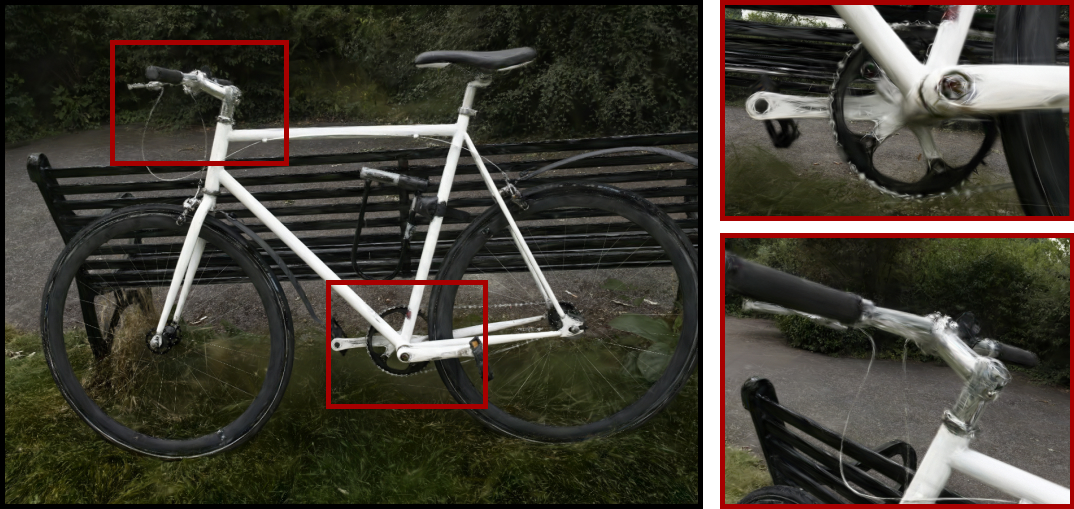
\includegraphics[width=0.9\textwidth]{Graphics/bici.jpg}
    \caption{Ejemplo visual de artefactos tipo ''aguja'' generados por la degeneración anisotrópica de gaussianas en \textit{Gaussian Splatting}. 
    En ambas ampliaciones se evidencia cómo ciertas 
    gaussianas adquieren formas extremadamente alargadas en direcciones específicas, generando artefactos visuales notorios que degradan 
    significativamente la calidad visual y comprometen la precisión geométrica de la reconstrucción.}
    \label{fig:bici}
\end{figure}

Una de las principales problemáticas asociadas al \textit{Gaussian Splatting} es la tendencia de las gaussianas a adquirir formas altamente anisotrópicas 
durante el proceso de optimización. Esto significa que, en lugar de mantener una forma más esférica o moderadamente elipsoidal, las gaussianas 
tienden a elongarse excesivamente en una dirección específica debido a una varianza dominante, generando artefactos visuales conocidos como agujas. 
Este comportamiento, reportado en estudios recientes  [\cite{hyung2024effectiverankanalysisregularization, huang2024spectralgstaming3dgaussian, yu2023mipsplattingaliasfree3dgaussian}],
no solo degrada la calidad visual de la reconstrucción, sino que también compromete la precisión de las normales estimadas, lo cual es crítico 
en tareas de iluminación realista y renderizado de alta calidad.
Además de esta degeneración geométrica, existe otra limitación importante: la incapacidad inherente del modelo para representar adecuadamente 
bordes abruptos, discontinuidades o superficies con cambios de curvatura pronunciados. Esta deficiencia proviene del hecho de que las gaussianas 
son distribuciones continuas por naturaleza, lo que las hace poco adecuadas para capturar transiciones bruscas en los datos visuales. Este fenómeno 
ha sido discutido en trabajos como \cite{qu2024discgsdiscontinuityawaregaussiansplatting}, donde se señala explícitamente que el 
uso exclusivo de gaussianas limita la capacidad del modelo para representar bordes definidos, afectando negativamente la reconstrucción 
de objetos con geometría compleja o detalles finos.

Cabe señalar que estas limitaciones no solo afectan la calidad visual, sino que también restringen la aplicabilidad del \textit{Gaussian Splatting} en 
contextos más exigentes, como reconstrucciones en tiempo real, modelado de escenas dinámicas, o aplicaciones donde la precisión geométrica es 
un factor determinante. En muchos casos, estas deficiencias obligan a recurrir a soluciones alternativas o a incorporar etapas adicionales de 
postprocesamiento que aumentan la complejidad y el costo computacional del sistema.

Por tanto, abordar esta problemática no es solo una cuestión de mejora estética o cuantitativa, sino una necesidad crítica para extender la 
utilidad práctica del \textit{Gaussian Splatting} a un espectro más amplio de aplicaciones. Resolver el problema de la forma subóptima de las gaussianas 
y su limitada capacidad de representación abre la puerta a métodos más robustos, adaptables y precisos.

\section{Antecedentes}
Existen diversas aproximaciones que han intentado resolver o mitigar las limitaciones mencionadas mediante modificaciones en la estructura 
fundamental de la gaussiana empleada en GS 
[\cite{qu2024discgsdiscontinuityawaregaussiansplatting, li20243d, huang2025deformableradialkernelsplatting,held20243dconvexsplattingradiance}]. 
Estas modificaciones buscan adaptar la forma, orientación o dispersión de las gaussianas para capturar mejor la complejidad geométrica de las escenas. 
No obstante, muchas de estas soluciones implican alteraciones significativas al pipeline original o introducen parámetros adicionales que aumentan la 
complejidad computacional y la demanda de memoria. 
Por esta razón, encontrar una solución que combine eficiencia computacional con mejoras sustanciales en la calidad visual y que a la vez sea adaptable 
a investigaciones realizadas sobre el \textit{Gaussian Splatting} original, sigue siendo un desafío relevante.

\section{Objetivos}

El objetivo general de esta tesis es desarrollar e implementar una modificación eficiente del método de \textit{Gaussian Splatting} 
que mejore significativamente la calidad visual y precisión geométrica en la representación de escenas tridimensionales mediante la 
introducción de parámetros basados en la asimetría o \textit{skewness}. 
Para lograr este objetivo, se plantean los siguientes objetivos específicos:

\begin{enumerate}
\item \textbf{Implementar un módulo eficiente de asimetría en Gaussian Splatting:}
\begin{itemize}
    \item Diseñar un esquema matemático que permita incorporar la asimetría de forma diferenciable dentro del algoritmo original.
    \item Programar un rasterizador diferenciable de gaussianas con asimetría el cual sea eficiente en cuanto a la memoria consumida y velocidad.
    \item Integrar el módulo desarrollado en el pipeline existente de Gaussian Splatting minimizando alteraciones significativas
     en la estructura original.
\end{itemize}

\item \textbf{Evaluar la mejora en la calidad visual y precisión geométrica:}
\begin{itemize}
    \item Crear un dataset que permita la evaluación del método propuesto utilizando recursos limitados.
    \item Evaluar la calidad visual utilizando métricas cuantitativas estándar (PSNR, SSIM, LPIPS) y compararlas con el Gaussian Splatting original.
    \item Validar la precisión geométrica midiendo la exactitud de las normales estimadas y la fidelidad geométrica mediante comparaciones con modelos de referencia.
\end{itemize}

\item \textbf{Optimizar la eficiencia computacional del método propuesto:}
\begin{itemize}
    \item Analizar el rendimiento del algoritmo modificado en términos de tiempo de ejecución y consumo de memoria en comparación con el método original.
    \item Realizar pruebas de rendimiento para garantizar que la implementación mantenga una tasa aceptable de fotogramas por segundo (FPS) en aplicaciones típicas.
    \item Documentar las compensaciones entre complejidad computacional y mejoras visuales obtenidas.
\end{itemize}

\item \textbf{Validar la aplicabilidad general del método propuesto:}
\begin{itemize}
    \item Probar la integración del método propuesto en diversas aplicaciones prácticas tales como renderizado en tiempo real, 
        reconstrucción de escenas dinámicas y modelado de objetos con alta complejidad geométrica.
    \item Comparar el método propuesto con soluciones alternativas existentes para destacar sus ventajas específicas y escenarios ideales de aplicación.
    \item Proporcionar un código fuente claro, modular y fácilmente extensible para facilitar su adopción en investigaciones futuras.
\end{itemize}
\end{enumerate}


\section{Propuestas de Solución}
La propuesta central de esta tesis consiste en incorporar un nuevo conjunto de parámetros que permitan añadir complejidad visual a la escena sin añadir
mucho coste computacional ni modificar abruptamente el método original para poder ser aplicado a investigaciones ya existentes que se basen en este. 
Debido a que al \textit{Gaussian Splatting} le cuesta representar discontinuidades tales como bordes de objetos o cambios
de color bruscos [\cite{qu2024discgsdiscontinuityawaregaussiansplatting}] y por ello tiende a crear gaussianas con formas de aguja para suplir esta carencia
[\cite{hyung2024effectiverankanalysisregularization, huang2024spectralgstaming3dgaussian,yu2023mipsplattingaliasfree3dgaussian}], 
hacer que las gaussianas posean bordes duros en una dirección entrenable podría resolver esta problemática. 
Además estos bordes duros podrian funcionar como una nueva normal de la mancha gaussiana, para ser aplicado en técnicas de iluminacion o reconstruccion de mallas.    

La asimetría o \textit{skewness} multivariante cumple las condiciones necesarias, por ello este trabajo busca introducirla en la distribución de las 
gaussianas tridimensionales utilizadas. Concretamente, se proponen cuatro nuevos parámetros: $s_x, s_y, s_z$ para definir 
la dirección y magnitud del desplazamiento en tres dimensiones de una segunda gaussiana idéntica a la original, y un parámetro adicional $S$, que 
controla la intensidad del efecto de asimetría. Esta modificación es implementada mediante la función:

\begin{equation}
    A \cdot (1-e^{-S \cdot B})
\end{equation}    

donde $B$ representa la gaussiana original $A$ desplazada por los parametros $s_x, s_y, s_z$. La elección de esta aproximación radica en su capacidad 
para introducir un corportamiento parecido a la asimetría sin modificar sustancialmente el algoritmo original de rasterización diferenciable.

\begin{figure}[htbp]
    \centering
    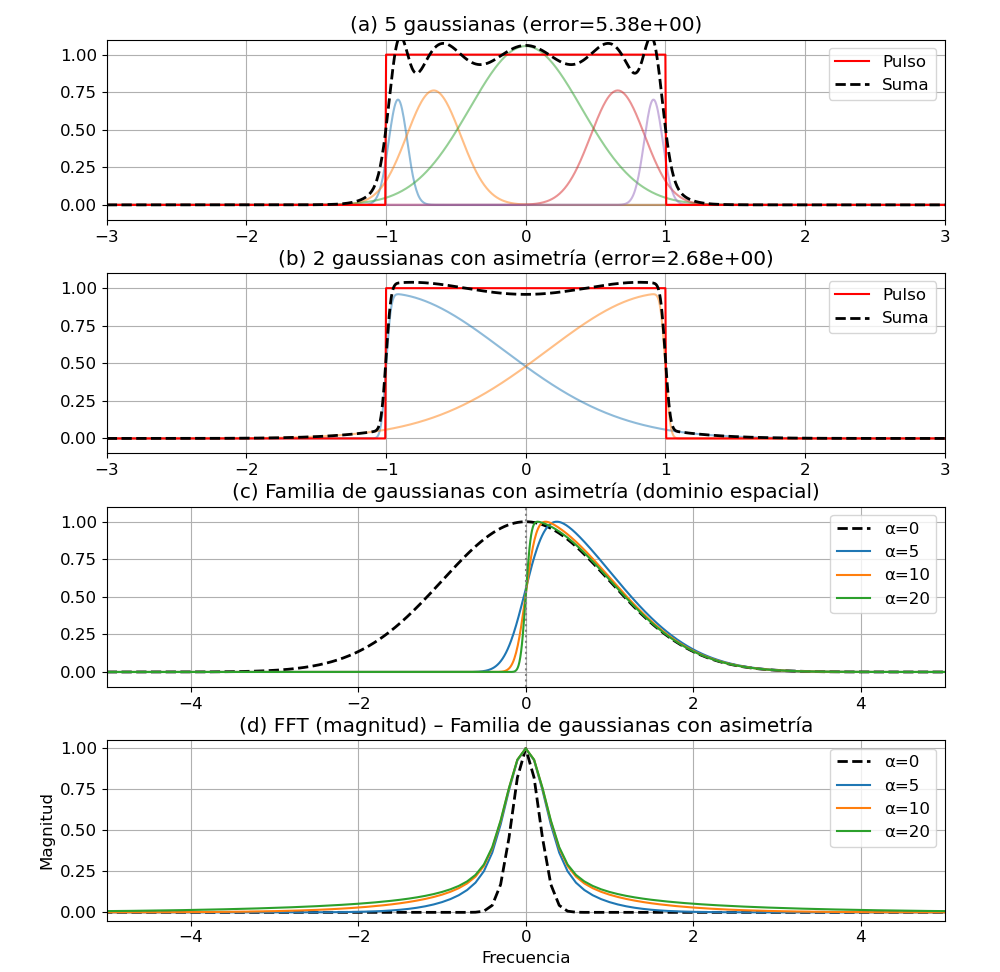
\includegraphics[width=1\textwidth]{Graphics/square_fft.png}
    \caption{Comparación entre gaussianas normales y gaussianas con asimetría en la aproximación de una señal cuadrada y sus respectivas transformadas de Fourier.   
    (a): Aproximación de un pulso cuadrado mediante la superposición de \(N = 5\) gaussianas simétricas optimizadas (error = 5.38). 
    (b): Aproximación del mismo pulso usando únicamente \(N = 2\) gaussianas con asimetría (error = 2.68), logrando una mejor representación de los bordes con menos componentes. 
    (c): Familia de gaussianas con diferentes niveles de asimetría en el dominio espacial para varios valores del parámetro \(\alpha\). A medida que \(\alpha\) aumenta, las funciones se inclinan hacia un lado, permitiendo mayor flexibilidad en la aproximación de funciones no simétricas. 
    (d): Magnitud de la transformada de Fourier (FFT) correspondiente a las funciones mostradas en (c), donde se observa que las gaussianas con asimetría presentan un mayor ancho de banda, lo que las hace más aptas para capturar componentes de alta frecuencia presentes en señales con transiciones abruptas.}
    \label{fig:square}
\end{figure}


\section{Estructura de la Tesis}
La tesis se organiza en los siguientes capítulos:
\begin{itemize}
    \item \textbf{Capítulo 2: Marco Teórico.} Se presentan conceptos fundamentales sobre espacios gaussianos, proyección y rasterización diferenciable, 
    y propiedades de distribuciones asimétricas.
    \item \textbf{Capítulo 3: Estado del Arte.} Se realiza una revisión crítica de \textit{Gaussian Splatting} y otros métodos relacionados, incluyendo técnicas 
    previas que abordan la modificación de las primitivas geométricas.
    \item \textbf{Capítulo 4: Metodología Propuesta.} Se detallan los aspectos teóricos y prácticos de la solución propuesta, incluyendo la simulación 
    de la asimetría y análisis de complejidad computacional.
    \item \textbf{Capítulo 5: Detalles de Implementación.} Se describen los componentes principales del código, incluyendo los kernels forward y backward 
    utilizados en el algoritmo de rasterización diferenciable propuesto.
    \item \textbf{Capítulo 6: Experimentos.} Se presentan hipótesis, diseño experimental, métricas de evaluación y resultados obtenidos tanto cuantitativos 
    como cualitativos.
    \item \textbf{Conclusiones y Recomendaciones.} Se resumen los aportes principales, limitaciones, aplicaciones potenciales y líneas futuras de 
    investigación sugeridas.
\end{itemize}


%\chapter{Marco Teórico}\label{chapter:theory}

\section{Espacios Gaussianos y representación en 3D}
\section{Proyección a 2D y rasterización diferenciable}
\section{Propiedades de las distribuciones sesgadas (skew-normal multivariante)}
\section{Notación y convenciones empleadas en la tesis}
\chapter{Estado del Arte}\label{chapter:state-of-the-art}

\section{Gaussian Splatting clásico}

\section{Representaciones basadas en Splatting}

\section{Otras representaciones volumétricas}

\section{Métodos de introducción de asimetría en modelado probabilístico}

\section{Comparación crítico-tabulada de eficiencia y calidad}

\chapter{Metodología propuesta}\label{chapter:proposal}

\section{Asimetría}

Como demuestran trabajos como \textit{3D-HGS} y \textit{Disc-GS}, abordar el problema de las discontinuidades en las superficies es fundamental para obtener mejores resultados de reconstrucción. Si bien enfoques como \textit{Convex Splatting}, \textit{DRK} y \textit{LinPrim} enfrentan este desafío mediante la modificación completa de la primitiva, ello conlleva incrementos considerables en el consumo de memoria y/o tiempo de cómputo, además de dificultar la integración de técnicas ya consolidadas sobre el framework original de \textit{Gaussian Splatting}. Por tal motivo, en este trabajo se propone utilizar la asimetría (\textit{skewness}) como mecanismo para resolver el problema, aprovechando que la función \textit{skew-normal} es una extensión natural de la función normal clásica. Esta función, al incorporar un parámetro de asimetría, permite modelar distribuciones con colas de diferente longitud y mayor flexibilidad, pero sin introducir una cantidad significativa de parámetros adicionales. Esto la hace especialmente adecuada para su implementación en \textit{pipelines} existentes.

\section{Simulación de la asimetría multivariante}

La forma propuesta de rasterizar una gaussiana con \textit{skewness} no reproduce técnicamente una función \textit{skew-normal} multivariante real, pero su comportamiento es análogo y cumple el mismo objetivo práctico, por lo que se hablará simplemente de asimetría en el contexto de este trabajo.

En la función \textit{skew-normal} en $\mathbb{R}^{3}$ se utilizan tres parámetros $\lambda$ que definen la dirección y magnitud de la asimetría. Para nuestra simulación se mantienen estos parámetros y, adicionalmente, se introduce un parámetro de sensibilidad $S$ que controla la nitidez del borde generado. Así, la nueva gaussiana rasterizada —siendo $A$ y $B$ dos gaussianas en $\mathbb{R}^{3}$ proyectadas a $\mathbb{R}^2$— se define mediante la siguiente fórmula:
\begin{equation}
    M = A \cdot (1 - e^{-S B})
    \label{eq:skew_mask}
\end{equation}
donde $B$ funciona como una máscara que determina la dirección del \textit{skewness} y define el borde duro. Específicamente, $B$ corresponde a la gaussiana $A$ trasladada por $\lambda$:
\[
B(x, y) = A\left(x - \lambda_x, y - \lambda_y\right)
\]
donde $\lambda \in \mathbb{R}^{2}$ es el vector de desplazamiento por \textit{skewness} en la imagen.

La elección de esta fórmula responde a la necesidad de crear un borde duro en un extremo de la primitiva y una cola suavizada en el otro. Visualmente, puede interpretarse como una pincelada que se desvanece: se genera una discontinuidad controlada en la opacidad, permitiendo tanto la creación de bordes definidos como la generación de gradientes o sombras del lado opuesto. Además, al estar compuesta únicamente por operaciones matemáticas básicas, la función resultante es diferenciable, lo que facilita su integración en flujos de trabajo optimizados y no requiere modificaciones profundas en el algoritmo de rasterización original.

\begin{figure}[htbp]
    \centering
    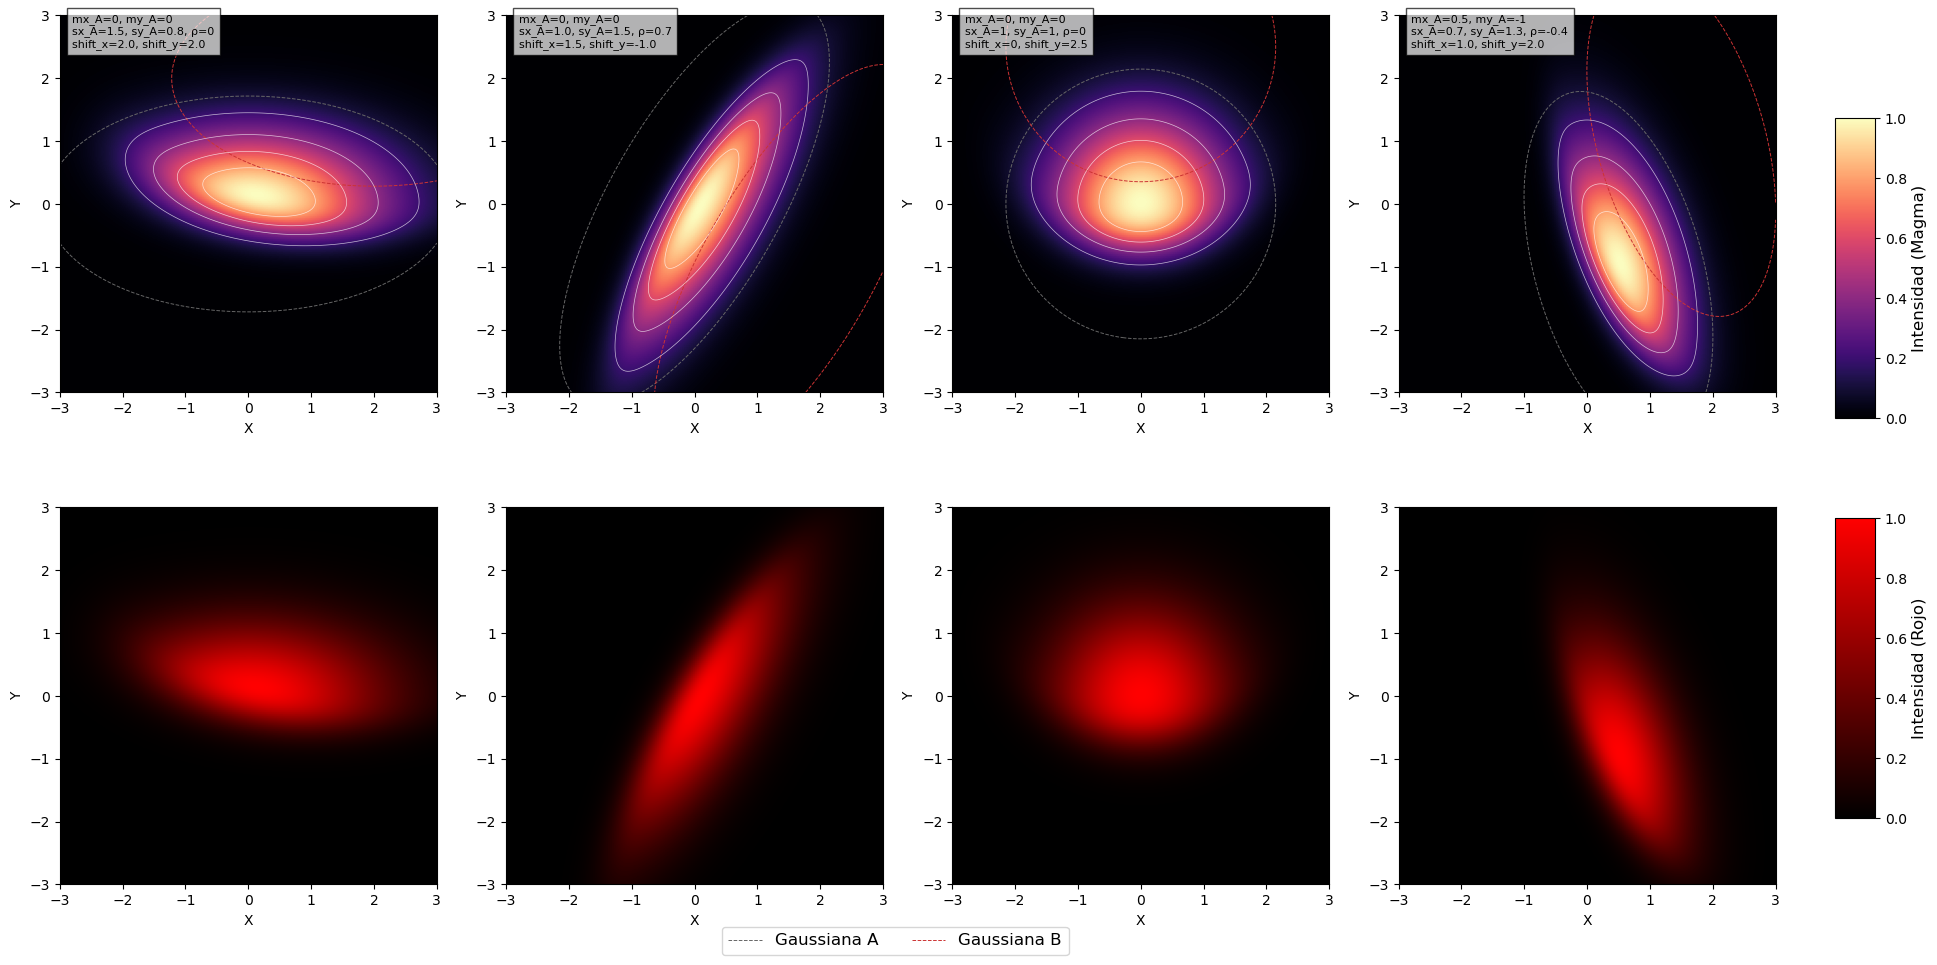
\includegraphics[width=1\textwidth]{Graphics/splatts.png}
    \caption{Visualización de la función de combinación \(A \cdot (1 - e^{-S B})\), utilizada para simular la asimetría. Se muestran cuatro configuraciones distintas de parámetros. La fila superior incluye mapas de calor con contornos de las gaussianas originales \(A\) y \(B\), mientras que la fila inferior muestra únicamente la distribución combinada en escala monocroma sobre fondo negro.}
    \label{fig:gaussianas_2d_skewness}
\end{figure}

Como $B$ es simplemente $A$ trasladada por $\lambda$, habiendo calculado:
\[
A_i(x, y) = \alpha_i^{\max} \exp\left(-\frac{1}{2}\mathbf{u}^{T}\mathbf{\Sigma}_i'^{-1}\mathbf{u}\right),
\]
siendo $\mathbf{u} = \begin{pmatrix} x \\ y \end{pmatrix} - \mathbf{x}_i$ y $\alpha_i^{\max}$ la opacidad máxima aprendida, sólo es necesario calcular además:
\[
B_i(x, y) = \exp\left(-\frac{1}{2}\mathbf{v}^{T}\mathbf{\Sigma}_i'^{-1}\mathbf{v}\right),
\]
donde $\mathbf{v} = \begin{pmatrix} x \\ y \end{pmatrix} - (\mathbf{x}_i - \lambda)$.
Posteriormente, se aplica la fórmula de combinación mediante la máscara:
\[
M_i(x, y) = A_i(x, y)\left[1 - \exp\left(-S B_i(x, y)\right)\right].
\]
El resto del algoritmo de rasterización se mantiene inalterado respecto a la versión clásica.

\section{Propagación de gradientes analítica}

Para implementar correctamente la optimización basada en gradientes, es necesario calcular de manera analítica las derivadas de la nueva función de máscara respecto a sus parámetros. Esto permite modificar el código de retropropagación (\textit{backward}) sin depender de aproximaciones numéricas.

\paragraph{Derivadas analíticas.}
%------------------------------------------------------------
%  Derivadas analíticas para el backward del “skew-splat”
%------------------------------------------------------------
\newcommand{\px}{x}\newcommand{\py}{y}
\newcommand{\dx}{d_x}\newcommand{\dy}{d_y}
\newcommand{\dlx}{d_x^{\lambda}}\newcommand{\dly}{d_y^{\lambda}}

\begin{align}
\mathbf{u} &= \begin{pmatrix}\px \\ \py\end{pmatrix}-\mathbf{x}_i,
&
\mathbf{v} &= \mathbf{u}-\boldsymbol{\lambda}_i,
\qquad
\boldsymbol{\lambda}_i=\begin{pmatrix}\lambda_{x,i}\\\lambda_{y,i}\end{pmatrix}
\\
A_i &= \alpha_i^{\max}\;
       \exp\!\Bigl(-\tfrac12\mathbf{u}^{\mathsf T}\mathbf{\Sigma}_i'\,\mathbf{u}\Bigr),
\label{eq:Adef}\\[2pt]
B_i &=       \exp\!\Bigl(-\tfrac12\mathbf{v}^{\mathsf T}\mathbf{\Sigma}_i'\,\mathbf{v}\Bigr),
\label{eq:Bdef}\\[2pt]
\alpha_i &= A_i\Bigl(1-e^{-S_i B_i}\Bigr).
\label{eq:alphadef}
\end{align}

%------------------------------------------------------------
\paragraph{Derivadas inmediatas de \(\alpha_i\)}%
\begin{align}
\frac{\partial\alpha_i}{\partial A_i} &= 1-e^{-S_i B_i},
&
\frac{\partial\alpha_i}{\partial B_i} &= A_i S_i e^{-S_i B_i},
&
\frac{\partial\alpha_i}{\partial S_i} &= A_i B_i e^{-S_i B_i}.
\label{eq:dalpha}
\end{align}

%------------------------------------------------------------
\paragraph{Derivadas de \(A_i\) }%
\begin{align}
\frac{\partial A_i}{\partial \alpha_i^{\max}}
  &= \frac{A_i}{\alpha_i^{\max}},
\\
\frac{\partial A_i}{\partial \Sigma'_{xx,i}}
  &= -\tfrac12\,\dx^{2}\,A_i,
&
\frac{\partial A_i}{\partial \Sigma'_{xy,i}}
  &= -\,\dx\dy\,A_i,
&
\frac{\partial A_i}{\partial \Sigma'_{yy,i}}
  &= -\tfrac12\,\dy^{2}\,A_i,
\\
\frac{\partial A_i}{\partial x_i}
  &= A_i\bigl(\Sigma'_{xx,i}\dx+\Sigma'_{xy,i}\dy\bigr),
&
\frac{\partial A_i}{\partial y_i}
  &= A_i\bigl(\Sigma'_{xy,i}\dx+\Sigma'_{yy,i}\dy\bigr).
\label{eq:dA}
\end{align}

%------------------------------------------------------------
\paragraph{Derivadas de \(B_i\)}%
\[
\dlx=\dx-\lambda_{x,i},\qquad
\dly=\dy-\lambda_{y,i}
\]

\begin{align}
\frac{\partial B_i}{\partial \Sigma'_{xx,i}}
  &= -\tfrac12\,\dlx^{2}\,B_i,
&
\frac{\partial B_i}{\partial \Sigma'_{xy,i}}
  &= -\,\dlx\dly\,B_i,
&
\frac{\partial B_i}{\partial \Sigma'_{yy,i}}
  &= -\tfrac12\,\dly^{2}\,B_i,
\\
\frac{\partial B_i}{\partial \lambda_{x,i}}
  &=  B_i\bigl(\Sigma'_{xx,i}\dlx+\Sigma'_{xy,i}\dly\bigr),
&
\frac{\partial B_i}{\partial \lambda_{y,i}}
  &=  B_i\bigl(\Sigma'_{xy,i}\dlx+\Sigma'_{yy,i}\dly\bigr),
\\
\frac{\partial B_i}{\partial x_i}
  &= -B_i\bigl(\Sigma'_{xx,i}\dlx+\Sigma'_{xy,i}\dly\bigr),
&
\frac{\partial B_i}{\partial y_i}
  &= -B_i\bigl(\Sigma'_{xy,i}\dlx+\Sigma'_{yy,i}\dly\bigr).
\label{eq:dB}
\end{align}

%------------------------------------------------------------
\paragraph{Derivada de la pérdida respecto a \(\alpha_i\)}

Para cada píxel \(p\) (y canal \(c\)), definimos la transmitancia
\(
T_{i-1,p}= \prod_{j<i}\bigl(1-\alpha_{j,p}\bigr)
\)
y el color acumulado antes de la primitiva \(i\) como
\(C_{p,c}^{\text{prev}}\).
Sea
\(g_{p,c}= \partial\mathcal{L}/\partial C_{p,c}\)
y, si se usa la regularización por profundidad,
\(h_p=\partial\mathcal{L}/\partial D_p\).
Entonces
\[
\frac{\partial\mathcal{L}}{\partial \alpha_{i,p}}
  =T_{i-1,p}\!\left[
      \sum_{c=1}^{C}\bigl(f_{i,c}-C_{p,c}^{\text{prev}}\bigr)g_{p,c}
      \;+\;
      \bigl(\tfrac1{d_i}-D_{p}^{\text{prev}}\bigr)h_{p}
    \right].
\label{eq:dLdalpha}
\]

Luego utilizando la regla de la cadena:

\begin{align}
\frac{\partial\mathcal{L}}{\partial f_{i,c}}
  &= \sum_{p}T_{i-1,p}\,\alpha_{i,p}\,g_{p,c},
\\
\frac{\partial\mathcal{L}}{\partial \alpha_i^{\max}}
  &=\sum_{p}
     \frac{\partial\mathcal{L}}{\partial\alpha_{i,p}}\;
     (1-e^{-S_i B_{i,p}})\,
     \frac{A_{i,p}}{\alpha_i^{\max}},
\\
\frac{\partial\mathcal{L}}{\partial S_i}
  &=\sum_{p}
     \frac{\partial\mathcal{L}}{\partial\alpha_{i,p}}\;
     A_{i,p} B_{i,p} e^{-S_i B_{i,p}},
\\
\frac{\partial\mathcal{L}}{\partial \lambda_{x,i}}
  &=\sum_{p}
     \frac{\partial\mathcal{L}}{\partial\alpha_{i,p}}\;
     A_{i,p}S_i e^{-S_i B_{i,p}}\,B_{i,p}\,
     \bigl(\Sigma'_{xx,i}\dlx+\Sigma'_{xy,i}\dly\bigr),
\end{align}

y análogamente para \(\lambda_{y,i}\),
los tres elementos \(\Sigma'_{xx,i},\Sigma'_{xy,i},\Sigma'_{yy,i}\)
y las coordenadas \(x_i,y_i\).



\section{Complejidad computacional y análisis de estabilidad numérica}

\subsection{Comparación de complejidad computacional}

El método propuesto introduce una ligera modificación sobre el \textit{Gaussian Splatting} clásico, pero mantiene la misma complejidad asintótica global. En el proceso de rasterización, mientras que el método clásico requiere únicamente una evaluación exponencial por cada píxel afectado (correspondiente a la gaussiana original), la versión con máscara \textit{skew} exige tres evaluaciones exponenciales por píxel: dos para las gaussianas $A$ y $B$ y una adicional para calcular la función de unión $1 - e^{-SB}$. Sin embargo, todas estas operaciones pueden fusionarse en un mismo núcleo de cálculo (\textit{kernel}), por lo que la penalización computacional resulta en un simple factor constante, típicamente en el rango de $1.8$ a $2.5$ veces el costo original en términos de operaciones de punto flotante (\textit{FLOPs}).

El resto de las etapas del algoritmo, incluyendo la composición alfa de los píxeles y la acumulación de resultados, se mantiene inalterado respecto al método clásico. Durante la fase de propagación de gradientes, se añaden derivadas respecto a los nuevos parámetros ($S$ y $\lambda$), pero el cálculo sigue siendo local y de complejidad constante por primitiva. Así, la complejidad global se mantiene en $O(Nk)$, donde $N$ es el número de primitivas gaussianas y $k$ el número de píxeles afectados por cada una.

En cuanto al consumo de memoria, la adición de los parámetros $S$ (sensibilidad) y $\lambda$ (vector de \textit{skewness}) implica un aumento marginal, ya que representan apenas cuatro números de punto flotante adicionales por cada primitiva. Este incremento suele ser despreciable en comparación con el resto de los atributos asociados a cada splat, como las texturas de armónicos esféricos.


\subsection{Estabilidad numérica de la modificación}

Al extender la formulación clásica con la máscara $A(1-e^{-SB})$, surgen algunas consideraciones sobre la estabilidad numérica de la implementación. En primer lugar, la función exponencial puede producir valores extremadamente pequeños cuando el argumento $SB$ es grande, lo que puede causar problemas de \textit{underflow} y anular los gradientes en regiones de opacidad muy alta. Para mitigar este efecto, se limitan los valores máximos de $S$ y se trabaja con precisión flotante simple (FP32).

En el extremo opuesto, cuando $SB$ es muy pequeño, la resta $1-e^{-SB}$ puede provocar cancelación numérica y pérdida de precisión, manifestándose en artefactos visuales de banda fina en los bordes de las primitivas. Este problema se evita reemplazando la operación por la función estándar \texttt{expm1}.

Otro posible inconveniente es la aparición de gradientes de gran magnitud, especialmente si $S$ crece sin restricciones, lo que puede desestabilizar el proceso de optimización durante el entrenamiento. Para mantener la estabilidad,se restringe el rango de $S$ mediante una función sigmoide acotada

Finalmente, como en el método clásico, es fundamental evitar que la matriz de covarianza $\Sigma$ adquiera valores demasiado pequeños, ya que esto puede provocar divisiones por casi cero y la aparición de “píxeles calientes” que dominan la función de pérdida. Esta situación se controla limitando los valores propios mínimos de $\Sigma$.


\chapter{Detalles de Implementación}\label{chapter:implementation}


Esta sección describe la extensión realizada sobre el \textit{pipeline} original de \textbf{3D Gaussian Splatting} para soportar la rasterización diferenciable de gaussianas con asimetría (\textit{skewness}). Para ello, se añadieron a cada gaussiana cuatro nuevos parámetros flotantes: \texttt{skew} y \texttt{skew\_sensitivity}. Nótese que \texttt{skew} está compuesto por tres parámetros (uno por cada eje espacial), mientras que \texttt{skew\_sensitivity} es un único valor escalar.

En el rasterizador diferenciable, la principal diferencia en la mayoría de los archivos es la inclusión de estas variables en las definiciones de entrada de múltiples funciones, hasta llegar al código del \textit{forward} y del \textit{backward} en CUDA, donde se ejecuta la lógica principal. Por esta razón, solo se explican detalladamente estos dos archivos, omitiendo el resto por considerarse cambios triviales.

Adicionalmente, se describe el código general del entrenamiento, que también se basa en el código original, con las modificaciones necesarias para incorporar la asimetría en el proceso de optimización.

\section{Rasterizador diferenciable de gaussianas con asimetría}
El rasterizador diferenciable de \textit{Gaussian Splatting} organiza su fase previa al pintado en varias etapas que se ejecutan íntegramente en la GPU. Primero, cada gaussiana de la escena se transforma con la matriz de vista y proyección para obtener una elipse en el plano de pantalla. A partir de esa elipse se calcula un rectángulo contenedor alineado con los ejes de la imagen que indica el rango de píxeles potencialmente afectados. Si dicho rectángulo queda fuera de los límites de la imagen o la opacidad asociada es insignificante, la gaussiana se descarta mediante \textit{culling} temprano, evitando trabajo posterior inútil.

Con los contenedores válidos se divide la imagen en \textit{tiles} regulares, por ejemplo de $16 \times 16$ píxeles, y se asigna un bloque de hilos CUDA a cada \textit{tile}. Para cada gaussiana se determina qué filas y columnas de \textit{tiles} intersecta su rectángulo; esos índices se almacenan en una lista global junto con un arreglo auxiliar que señala, para cada \textit{tile}, la posición inicial y la cantidad de gaussianas que le corresponden. 

Antes de la rasterización por píxel, las gaussianas asociadas a cada \textit{tile} se ordenan por profundidad, utilizando como clave la coordenada z del centro proyectado. Esta ordenación garantiza que, cuando se componga la opacidad, el resultado sea consistente con la lógica de \textit{front-to-back}.

Con las listas ya ordenadas se preparan buffers locales en memoria compartida para transmittancia parcial, máscaras y cualquier dato intermedio que se necesite durante el cómputo del \textit{tile}. Parámetros constantes como la inversa de la matriz de proyección o factores globales de escala se copian a memoria constante de la GPU para reducir la latencia de lectura.

Por último se lanza un \textit{kernel} dedicado a cada \textit{tile}; dentro de él, cada hilo procesa uno o varios píxeles del \textit{tile}. Ese \textit{kernel} realiza la evaluación de las gaussianas y la composición alfa de forma diferenciable, su funcionamiento sera explicado en las proximas secciones. Es importante notar que todas las etapas previas son transformaciones deterministas y continuas respecto a los parámetros de cada gaussiana, por lo que los marcos de autograd pueden propagar gradientes sin interrupciones.


\subsection{Kernel Forward}
\subsection{Kernel \texttt{Forward} con soporte para asimetría}

En el \textit{kernel} \texttt{forward} del rasterizador se programan modificaciones específicas para incorporar soporte a la asimetría, mediante la proyección de una segunda gaussiana desplazada y la aplicación de la máscara diferenciable basada en dicha proyección. Los principales cambios ocurren en las funciones  \texttt{preprocessCUDA} y \texttt{renderCUDA} del archivo \texttt{cuda\_rasterizer/forward.cu}, estas dos fases son llamadas secuencialmente al rasterizar. 

\paragraph{Preprocesamiento}
Durante esta fase, se transforma el centro de cada gaussiana, así como el punto desplazado por el vector \texttt{skew}. Ambos se proyectan al plano de la imagen, y se calcula la diferencia de posición en píxeles, que se almacena como \texttt{skews2D}. Esta diferencia servirá posteriormente para computar la máscara. El siguiente fragmento muestra el código relevante añadido en \texttt{preprocessCUDA}:


\begin{minted}[bgcolor=bgcode, linenos, fontsize=\footnotesize]{cpp}
// Transformación del punto desplazado por skew
float3 p_skew_world = {
    p_orig.x + skews[idx].x,
    p_orig.y + skews[idx].y,
    p_orig.z + skews[idx].z
};

float4 p_skew_h = transformPoint4x4(p_skew_world, projmatrix);

float inv_w_skew = 1.f / (p_skew_h.w + 1e-7f);
float2 p_skew_pix = {
    ndc2Pix(p_skew_h.x * inv_w_skew, W),
    ndc2Pix(p_skew_h.y * inv_w_skew, H)
};

skews2D[idx] = {
    p_skew_pix.x - point_image.x,
    p_skew_pix.y - point_image.y
};
\end{minted}

\paragraph{Rasterización por píxel}
En esta etapa, cada hilo evalúa una o varias gaussianas sobre su píxel correspondiente. Se computa tanto la gaussiana original como una versión desplazada, y se estima la máscara suavizada que modula la opacidad. El cálculo se basa en la forma:  


\[
\alpha = A \cdot \left(1 - \exp(-S \cdot B)\right)
\]

donde $A$ es la evaluación de la gaussiana original, $B$ es la misma gaussiana pero desplazada, y $S$ es el parámetro \texttt{skew\_sensitivity}. A continuación se muestra el codigo modificado en \texttt{renderCUDA} :



\begin{minted}[bgcolor=bgcode, linenos, fontsize=\footnotesize]{cpp}
// --- Se evalúa A: Gaussiana en el píxel actual ---
float power = fmaf(-0.5f, 
                  (con_o.x * d.x*d.x + con_o.z * d.y*d.y),
                   - con_o.y * d.x * d.y);
if (power > 0.0f)
    continue;
float A = con_o.w * expf(power);

// --- Se evalúa B: misma Gaussiana desplazada por skew ---
int   id     = collected_id[j];
float sx = skews2D[id].x;
float sy = skews2D[id].y;

float2 dB    = { d.x - sx, d.y - sy };
float powerB = fmaf(-0.5f , 
                   (con_o.x * dB.x*dB.x+ con_o.z * dB.y*dB.y),
                    - con_o.y * dB.x * dB.y);
float B = expf(powerB);

// --- Se aplica la máscara de asimetría ---
float mask      = -expm1f(-skew_sensitivity[id] * B);
float alpha = min(0.99f, A*mask);
\end{minted}

Se utilizan las funciones \texttt{fmaf} y \texttt{expm1f} para mejorar la precisión numérica del cálculo. La función \texttt{fmaf} realiza una multiplicación y una suma en una sola operación con redondeo único, reduciendo errores de acumulación. Por su parte, \texttt{expm1f} computa $\exp(x) - 1$ con mayor precisión cuando $x$ es cercano a cero, lo cual evita la cancelación numérica que ocurre al restar dos números casi iguales.

\subsection{Kernel Backward}


El \textit{kernel backward} se encarga de calcular las derivadas necesarias para propagar los gradientes durante el entrenamiento, considerando las modificaciones introducidas por el modelo con asimetría. Este kernel está compuesto por dos funciones principales: \texttt{preprocessCUDA} y \texttt{renderCUDA}, las cuales son ejecutadas de forma inversa al forward.

La función \texttt{preprocessCUDA} calcula la derivada del centro tridimensional de cada gaussiana proyectada, y adicionalmente propaga el gradiente hacia los parámetros \texttt{skew} y \texttt{skew\_sensitivity}. Para ello, transforma tanto el centro original como el punto desplazado por \texttt{skew} al espacio de imagen, y computa cómo las variaciones en las posiciones 2D afectan las coordenadas 3D originales, considerando la proyección con perspectiva. Este procedimiento permite calcular cómo pequeñas variaciones en los parámetros de asimetría afectan la imagen final.

Por su parte, la función \texttt{renderCUDA} computa las derivadas respecto a todos los parámetros relevantes durante el proceso de rasterización diferenciable. Para cada píxel afectado, se evalúan tanto la gaussiana original como la desplazada, y se calcula la contribución de cada una a la opacidad final utilizando la máscara de asimetría. El gradiente de la pérdida con respecto al valor del píxel se propaga hacia:

\begin{itemize}
    \item Las coordenadas del centro proyectado (\texttt{mean2D}).
    \item Los coeficientes de la matriz cónica de opacidad (\texttt{conic2D}).
    \item La posición relativa del desplazamiento en 2D (\texttt{skews2D}).
    \item La sensibilidad del \texttt{skew} (\texttt{skew\_sensitivity}).
    \item La opacidad base de la gaussiana.
    \item El color y la profundidad inversa si están presentes.
\end{itemize}

Este cálculo tiene en cuenta la acumulación alfa (\textit{alpha compositing}) en orden de profundidad, lo cual es crucial para que los gradientes se correspondan con el modelo de formación de imagen usado en la fase \texttt{forward}. Las contribuciones de cada parámetro son diferenciadas y acumuladas mediante operaciones atómicas, asegurando la corrección numérica en entornos altamente paralelos.

Finalmente, los gradientes sobre \texttt{skews2D} se transforman nuevamente a coordenadas tridimensionales en la función \texttt{preprocessCUDA}, completando así la ruta de retropropagación desde la imagen generada hacia los parámetros originales de cada gaussiana. Este diseño permite integrar la asimetría como un componente completamente diferenciable dentro del pipeline de entrenamiento de \textit{3D Gaussian Splatting}.

\section{Optimización de hiperparámetros}
\label{sec:hyperopt}

Durante la extensión del rasterizador diferenciable para soportar gaussianas asimétricas, se observó que la incorporación de nuevos parámetros, así como las modificaciones en la lógica del \textit{forward} y \textit{backward}, provocaron un cambio significativo en la escala y la dinámica de los gradientes propagados a lo largo del \textit{pipeline}. En particular, algunos gradientes asociados a los parámetros de posición, escala y opacidad se incrementaron hasta dos órdenes de magnitud respecto al pipeline original, lo que resultó en una sensibilidad marcada en la elección de los hiperparámetros de entrenamiento. Por tanto, fue imprescindible realizar una reoptimización cuidadosa de todos los hiperparámetros principales.

Para abordar este problema, se diseñó una estrategia de optimización de hiperparámetros basada en \textbf{Optuna}, el cual emplea algoritmos bayesianos para explorar el espacio de búsqueda de manera adaptativa. La optimización se realizó sobre los principales hiperparámetros de entrenamiento: tasas de aprendizaje (para posición, opacidad, escala, rotación y \textit{features}), umbrales y frecuencias de densificación, así como parámetros de regularización. 

Cada combinación candidata de hiperparámetros fue evaluada en múltiples escenas. Como métrica objetivo se utilizó el \textit{Peak Signal-to-Noise Ratio} (PSNR) promedio entre todas las escenas, incentivando la consistencia entre dominios. Para reducir el coste computacional y evitar el sobreajuste, se implementó \textit{early stopping} basado en la evolución del PSNR y un umbral mínimo de mejora significativa. Además, se estableció un límite de tiempo para cada prueba y se empleó \textit{pruning} de los experimentos poco prometedores.

\subsection{Parámetros optimizados y resultados}

Como resultado de este proceso, se obtuvo una configuración de hiperparámetros óptima que permitió estabilizar y maximizar la calidad de reconstrucción visual del modelo con asimetría, logrando valores de PSNR superiores y evitando oscilaciones no deseadas durante el entrenamiento. Los valores finales seleccionados para los principales hiperparámetros del modelo asimétrico fueron los siguientes:\footnote{Los nombres corresponden a los argumentos de la clase \texttt{OptimizationParams}.}

\begin{center}
\begin{tabular}{ll}
\toprule
\textbf{Hiperparámetro} & \textbf{Valor óptimo} \\
\midrule
\texttt{position\_lr\_init}           & $3.79 \times 10^{-4}$ \\
\texttt{position\_lr\_final}          & $3.35 \times 10^{-7}$ \\
\texttt{position\_lr\_delay\_mult}    & $4.68 \times 10^{-2}$ \\
\texttt{feature\_lr}                  & $1.25 \times 10^{-5}$ \\
\texttt{opacity\_lr}                  & $7.49 \times 10^{-2}$ \\
\texttt{scaling\_lr}                  & $2.50 \times 10^{-2}$ \\
\texttt{rotation\_lr}                 & $2.31 \times 10^{-3}$ \\
\bottomrule
\end{tabular}
\end{center}

\noindent
Cabe señalar que los valores encontrados difieren notablemente de los empleados en el pipeline original, reflejando el impacto de la nueva parametrización y la necesidad de ajustar las escalas de aprendizaje para cada tipo de parámetro. En particular, el \textit{learning rate} para opacidad y escala resultó significativamente mayor, compensando la reducción relativa de gradiente en estos parámetros tras la incorporación de la asimetría.


\chapter{Experimentos}\label{chapter:experiments}

\section{Hipótesis a validar}

El objetivo central de este trabajo es validar la hipótesis de que extender las gaussianas empleadas en el algoritmo de \emph{Gaussian Splatting} para incorporar formas asimétricas, mediante la introducción de un parámetro de \emph{skewness}, permite una representación más fiel y expresiva de escenas tridimensionales. A diferencia de las gaussianas tradicionales, que presentan bordes difuminados y simétricos, las gaussianas asimétricas propuestas permiten simular colas alargadas y bordes más definidos, características que podrían ser determinantes en la reconstrucción precisa de superficies con límites abruptos o transiciones de color pronunciadas.

Esta generalización no solo busca mejorar la reconstrucción visual en términos de métricas objetivas como \emph{PSNR}, \emph{SSIM} y \emph{LPIPS}, sino también explorar la posibilidad de que el borde más rígido inducido por la asimetría pueda actuar como una estimación de la normal local a la superficie representada. Tal propiedad podría ser explotada en aplicaciones posteriores, tales como la generación de mallas poligonales a partir de nubes gaussianas, técnicas de sombreado y estimación de iluminación basada en normales. En consecuencia, se pretende evaluar no solo la capacidad de estas gaussianas asimétricas para representar con mayor precisión tanto bordes duros como gradientes suaves, sino también su potencial utilidad como entidades geométricas intermedias en tareas de reconstrucción y renderizado más avanzadas.

\section{Diseño experimental}

La experimentación se ve condicionada por la disponibilidad de recursos computacionales, en particular la imposibilidad de acceder a una GPU con 24\,GB de memoria, cantidad recomendada para la ejecución eficiente de algoritmos de \emph{Gaussian Splatting} sobre conjuntos de datos clásicos como \emph{Mip-NeRF 360} y \emph{Tanks \& Temples}. Por este motivo, se decide la construcción de un conjunto de datos propio, optimizado para un consumo de memoria reducido, que permitia la validación experimental en hardware más modesto sin sacrificar la representatividad de las escenas.

\subsection{UH-Statues Dataset}

El conjunto de datos creado, denominado \textbf{UH-Statues Dataset}, se compone por 7 escenas distintas (\emph{poey}, \emph{owl}, \emph{almamater}, \emph{urn}, \emph{benito}, \emph{humboldt}, \emph{einstein}), cuidadosamente seleccionadas para cubrir tanto ambientes interiores (\emph{urn} y \emph{poey}) como exteriores. En todos los casos, la captura se realiza apuntando la cámara hacia un objeto principal, siendo en su mayoría estatuas localizadas en la Universidad de La Habana: cinco de ellas situadas en la Facultad de Matemática y Computación y una en la Facultad de Física. La selección de escenas se diseña para garantizar diversidad en la iluminación y el fondo, a la vez que se mantenía el enfoque en un único objeto de interés, lo que facilita el entrenamiento y evaluación del algoritmo.

\begin{figure}[htbp]
    \centering
    \includegraphics[width=1.0\textwidth]{Graphics/dataset.png}
    \caption{Escenas del dataset UH-Statues, de izquierda a derecha las escenas: poey, owl, almamater, benito, urn, humboldt, einstein.}
    \label{fig:dataset}
\end{figure}

La captura de los datos se realiza utilizando un \textbf{iPhone 15} en modo video estándar, con resolución 4K a 30\,\emph{fps}, sin aplicar \emph{zoom}, y utilizando exclusivamente la cámara principal, la cual posee una distancia focal de 26\,mm. La duración de cada video no supera el minuto, lo que limita la cantidad de imágenes a procesar y, en consecuencia, reduce significativamente el consumo de memoria durante el entrenamiento del modelo.

\paragraph{Preprocesamiento y reconstrucción}
El pipeline de preprocesamiento para cada escena consiste en los siguientes pasos:
\begin{enumerate}
    \item \textbf{Extracción de imágenes:} De cada video se extraen 2 fotogramas por segundo, obteniendo así un conjunto de imágenes suficientemente representativo de la escena, pero evitando la redundancia asociada a una mayor frecuencia de muestreo.
    \item \textbf{Transformación y escalado:} Las imágenes extraídas son transpuestas para garantizar una orientación uniforme y redimensionadas a un ancho fijo de 1920 píxeles, manteniendo la relación de aspecto original. Esta reducción de resolución es clave para disminuir el consumo de memoria y acelerar el procesamiento subsiguiente.
    \item \textbf{Reconstrucción de la cámara:} La calibración y reconstrucción de la geometría de la escena se realizó utilizando \textbf{COLMAP}, especificando que las imágenes son tomadas con una cámara tipo \emph{pinhole} y distorsión radial/tangencial siguiendo el modelo de OpenCV. COLMAP [\cite{schonberger2016structure}] es una herramienta robusta para la reconstrucción tridimensional a partir de imágenes, que estima tanto las posiciones relativas de las cámaras como una nube de puntos 3D de la escena. El resultado de COLMAP incluye los parámetros intrínsecos y extrínsecos de la cámara para cada imagen, así como una reconstrucción inicial de la estructura 3D, información que posteriormente se emplea como entrada para el algoritmo de \emph{Gaussian Splatting}.
\end{enumerate}

\paragraph{Ventajas de este dataset}
La principal ventaja del \emph{UH-Statues Dataset} radica en su bajo consumo de memoria durante el entrenamiento, consecuencia directa de:
\begin{itemize}
    \item El número reducido de imágenes por escena, derivado tanto de la corta duración de los videos como de la baja frecuencia de muestreo de fotogramas.
    \item La resolución moderada de las imágenes, que limita el tamaño de los mapas de proyección y los buffers intermedios utilizados durante la rasterización.
    \item La simplicidad de las escenas, en las que predomina un único objeto de interés y fondos poco recargados, lo que reduce la necesidad de una gran cantidad de gaussianas para una reconstrucción precisa.
\end{itemize}
Este diseño permite ejecutar el pipeline completo de \emph{Gaussian Splatting} en GPUs con capacidad de memoria limitada, a diferencia de datasets más complejos y de mayor tamaño, como \emph{Mip-NeRF 360}, donde la cantidad de imágenes y la resolución implican requerimientos significativamente más altos.

\section{Métricas de evaluación}

Para cuantificar la calidad de las reconstrucciones obtenidas mediante los diferentes modelos, se emplean las métricas objetivas estándar en la literatura de síntesis y reconstrucción de imágenes: \textbf{PSNR}, \textbf{SSIM} y \textbf{LPIPS}. Estas métricas han demostrado ser indicadores confiables del parecido visual entre la imagen generada y la imagen real, y son ampliamente utilizadas tanto en los trabajos fundacionales de \emph{Gaussian Splatting} [\cite{kerbl20233d}] como en métodos derivados.

\subsection{PSNR (Peak Signal-to-Noise Ratio)}
El \emph{PSNR} es una métrica tradicionalmente utilizada para evaluar la calidad de imágenes reconstruidas, definida en función del error cuadrático medio (\emph{MSE}) entre la imagen generada y la imagen de referencia. Matemáticamente, se expresa como:
\begin{equation}
    \mathrm{PSNR} = 10 \cdot \log_{10} \left( \frac{MAX_I^2}{\mathrm{MSE}} \right)
\end{equation}  

donde $MAX_I$ es el valor máximo posible de un píxel en la imagen. Un mayor valor de PSNR indica mayor similitud entre las imágenes. Esta métrica es sensible a pequeños errores de reconstrucción y ha sido utilizada extensivamente en la literatura de procesamiento de imágenes [\cite{huynh2008scope}].

\subsection{SSIM (Structural Similarity Index)}
El \emph{SSIM} [\cite{wang2004image}] es una métrica perceptual que evalúa la similitud estructural entre dos imágenes, considerando luminancia, contraste y estructura. Se calcula mediante:
\begin{equation}
    \mathrm{SSIM}(x, y) = \frac{(2\mu_x\mu_y + c_1)(2\sigma_{xy} + c_2)}{(\mu_x^2 + \mu_y^2 + c_1)(\sigma_x^2 + \sigma_y^2 + c_2)}
\end{equation}
donde $\mu_x$, $\mu_y$ son las medias, $\sigma_x^2$, $\sigma_y^2$ las varianzas, y $\sigma_{xy}$ la covarianza local de las ventanas comparadas en cada imagen. SSIM produce valores entre $-1$ y $1$, siendo $1$ el máximo de similitud.

\subsection{LPIPS (Learned Perceptual Image Patch Similarity)}
\emph{LPIPS} [\cite{zhang2018unreasonable}] es una métrica aprendida, que mide la distancia perceptual entre imágenes utilizando activaciones intermedias de redes neuronales profundas entrenadas para reconocimiento de imágenes. A diferencia de PSNR y SSIM, LPIPS se correlaciona mejor con la percepción humana de similitud visual, especialmente en contextos de reconstrucción de imágenes complejas o sintéticas. Valores bajos de LPIPS indican mayor similitud perceptual entre la imagen generada y la de referencia.




\section{Resultados Cuantitativos}

Se entrenó un modelo para cada escena del dataset desarrollado, realizando 15000 iteraciones para cada una. En la mayoría de las escenas se aplicó un proceso de densificación cada 100 iteraciones hasta alcanzar las primeras 1000 iteraciones. Excepcionalmente, las escenas denominadas \textit{poey} y \textit{owl} pudieron densificarse hasta la iteración 5000, debido al menor consumo de memoria en la GPU. Todos los experimentos se realizan en una Nvidia RTX 4060 Max-Q de 8\,GB.

La comparación directa entre el método propuesto, \textbf{Directional Asymmetric Gaussian Splatting (DA-GS)}, y el método original, se presenta en la Figura~\ref{tab:quality_dags_vs_vanilla}. Se muestran las métricas Peak Signal-to-Noise Ratio (PSNR), Structural Similarity Index Measure (SSIM), Learned Perceptual Image Patch Similarity (LPIPS), así como el número final de puntos en cada modelo entrenado (Pts).

\begin{table}[h!]
    \centering
    \resizebox{\textwidth}{!}{%
    \begin{tabular}{@{}lcccc cccc@{}}
        \toprule
        & \multicolumn{4}{c}{\textbf{DA-GS}}
        & \multicolumn{4}{c}{\textbf{Vanilla GS}} \\
        \cmidrule(lr){2-5}\cmidrule(lr){6-9}
        Escena & PSNR$\uparrow$ & SSIM$\uparrow$ & LPIPS$\downarrow$ & Pts$\downarrow$
               & PSNR$\uparrow$ & SSIM$\uparrow$ & LPIPS$\downarrow$ & Pts$\downarrow$ \\
        \midrule
        poey       & --    & -- & -- & --         & 33.20 & -- & -- & 2,390,147 \\
        almamater  & 24.45 & -- & -- & \textbf{72,557} & 25.22 & -- & -- & 73,762 \\
        owl        & 24.12 & -- & -- & \textbf{1,356,670} & 24.87 & -- & -- & 2,238,576 \\
        humboldt   & 18.13 & -- & -- & 27,423         & 18.81 & -- & -- & \textbf{26,388} \\
        benito     & 23.68 & -- & -- & \textbf{731,137} & 24.32 & -- & -- & 750,608 \\
        urn        & 27.50 & -- & -- & 22,234         & 30.32 & -- & -- & \textbf{20,604} \\
        einstein   & --    & -- & -- & --             & --    & -- & -- & -- \\
        \bottomrule
    \end{tabular}}
    \caption{Comparación de calidad entre \textbf{DA-GS} y \textbf{Vanilla GS}. Para PSNR y SSIM, valores más altos son mejores ($\uparrow$); para LPIPS y el número final de puntos (Pts) valores más bajos son mejores ($\downarrow$).}
    \label{tab:quality_dags_vs_vanilla}
\end{table}

Además, se realiza una comparación adicional para validar el comportamiento del \textbf{DA-GS} cuando se congela el parámetro de asimetría en 0, esperado a comportarse de manera similar al método original del \textbf{GS}. Estos resultados se presentan en la Figura~\ref{tab:quality_dags_vs_skewfrozen}.

\begin{table}[H]
    \centering
    \resizebox{\textwidth}{!}{%
    \begin{tabular}{@{}lcccc cccc@{}}
        \toprule
        & \multicolumn{4}{c}{\textbf{DA-GS}}
        & \multicolumn{4}{c}{\textbf{DA-GS (skew frozen)}} \\
        \cmidrule(lr){2-5}\cmidrule(lr){6-9}
        Escena & PSNR$\uparrow$ & SSIM$\uparrow$ & LPIPS$\downarrow$ & Pts$\downarrow$
               & PSNR$\uparrow$ & SSIM$\uparrow$ & LPIPS$\downarrow$ & Pts$\downarrow$ \\
        \midrule
        poey       & --    & -- & -- & --             & 32.81 & -- & -- & 2,605,931 \\
        almamater  & \textbf{24.45} & -- & -- & \textbf{72,557}         & 24.43 & -- & -- & 73,698 \\
        owl        & \textbf{24.12} & -- & -- & \textbf{1,356,670}      & 23.71 & -- & -- & 2,165,915 \\
        humboldt   & 18.13 & -- & -- & \textbf{27,423}         & \textbf{18.29} & -- & -- & 28,145 \\
        benito     & 23.68 & -- & -- & 731,137        & --    & -- & -- & -- \\
        urn        & 27.50 & -- & -- & 22,234         & \textbf{27.78} & -- & -- & \textbf{22,051} \\
        einstein   & --    & -- & -- & --             & --    & -- & -- & -- \\
        \bottomrule
    \end{tabular}}
    \caption{Comparación de calidad entre \textbf{DA-GS} y \textbf{DA-GS con skewness congelado}. Para PSNR y SSIM, valores más altos son mejores ($\uparrow$); para LPIPS y Pts valores más bajos son mejores ($\downarrow$).}
    \label{tab:quality_dags_vs_skewfrozen}
\end{table}

\section{Resultados Cualitativos}

Para validar cualitativamente la hipótesis de que las gaussianas con asimetría explotan sus bordes más definidos para modelar bordes en objetos tridimensionales, se procede a colorear las gaussianas según la dirección del vector de asimetría. Estos resultados son comparados visualmente con las normales obtenidas de la implementación original del \textit{Gaussian Splatting}, las cuales son extraídas a partir de la dirección de menor varianza de cada gaussiana. La comparación visual de ambos métodos puede apreciarse en la Figura~\ref{fig:normals}.

\begin{figure}[htbp]
\centering
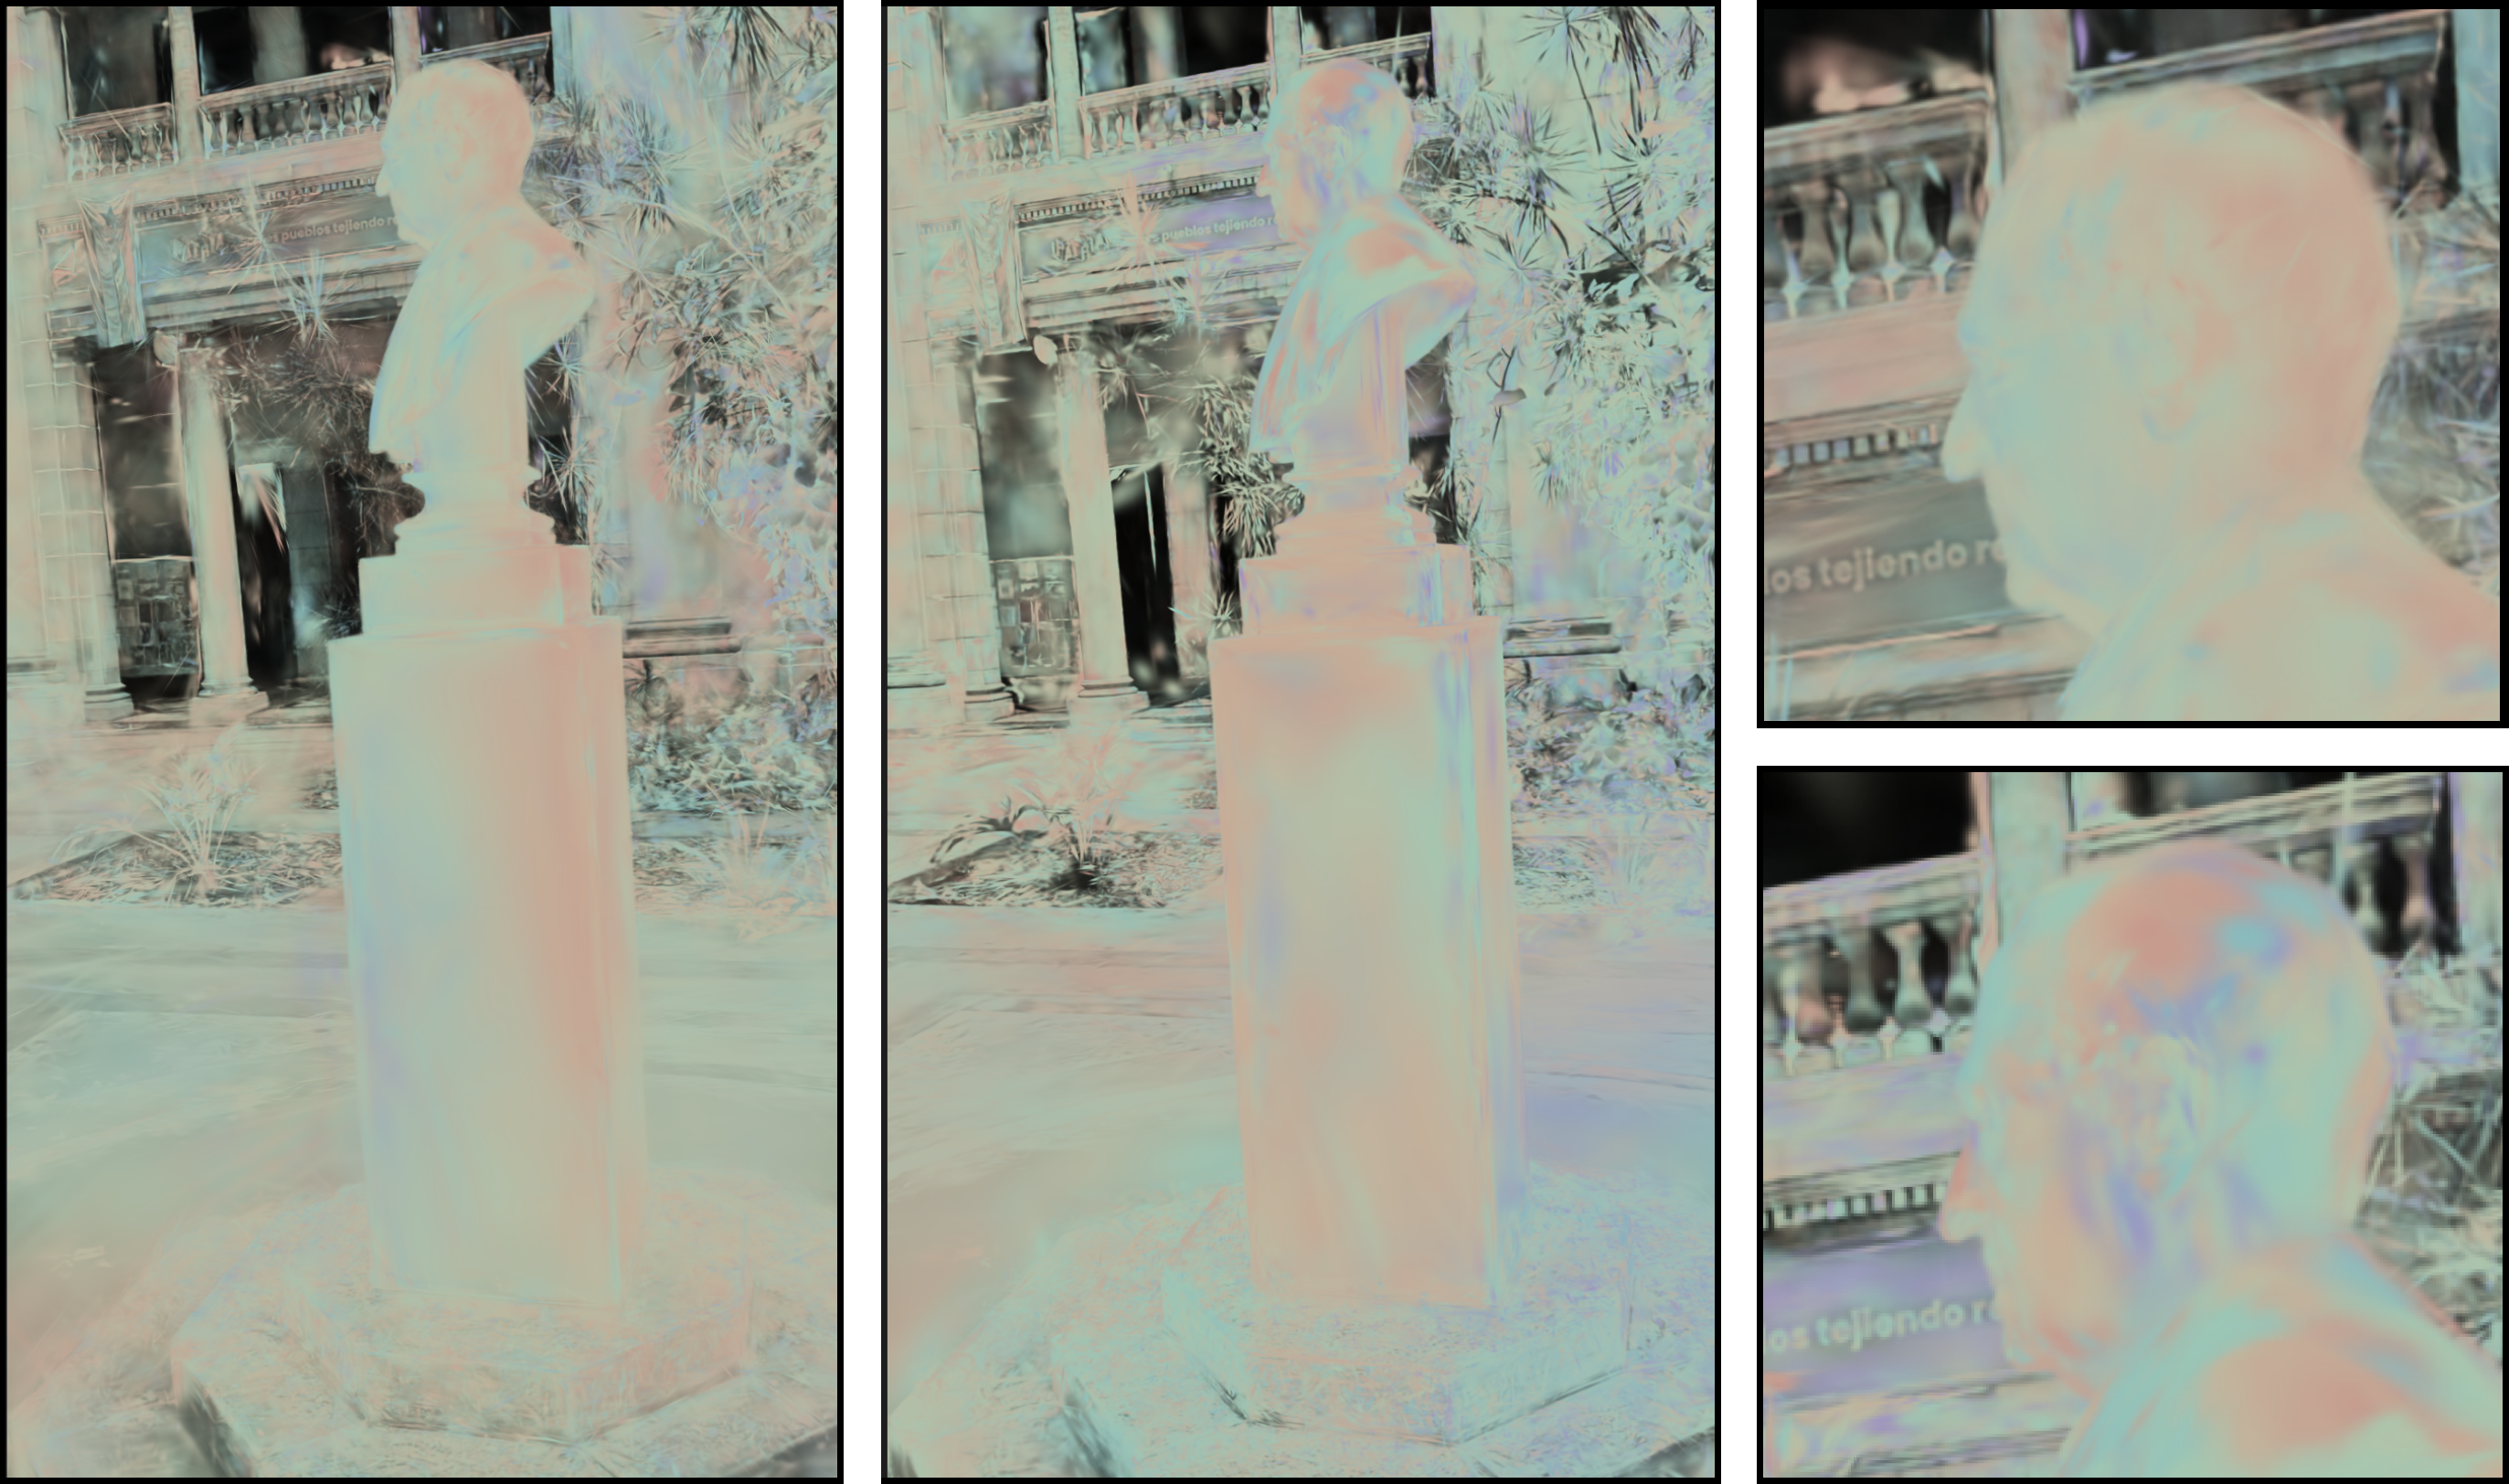
\includegraphics[width=1.0\textwidth]{Graphics/normals.png}
\caption{Comparación visual de la dirección del vector de asimetría (izquierda) y las normales estimadas por el \textit{Gaussian Splatting} original (derecha). Modelos entrenados sobre la escena \textit{poey}, a 5000 iteraciones.}
\label{fig:normals}
\end{figure}

\subsubsection{Análisis y discusión}


Los resultados obtenidos revelan que si bien, en términos absolutos, no se alcanzan los resultados del \textit{Gaussian Splatting} original, se evidencia que la incorporación del parámetro de asimetría aporta beneficios medibles. Al comparar la versión completa del modelo con la variante en la que el parámetro de \textit{skewness} se congela en cero, se observa de manera consistente que el uso de gaussianas asimétricas mejora los resultados. Esto respalda la hipótesis fundamental de este trabajo: que la introducción de direccionalidad permite una mejor adaptación local a la geometría de la escena, particularmente en regiones con bordes o discontinuidades.

Sin embargo, un hallazgo relevante es que incluso al congelar el parámetro de asimetría, con lo cual el modelo debería comportarse de manera análoga al GS original, se obtienen resultados inferiores. Esta observación sugiere que el modelo DA-GS posee dinámicas de entrenamiento diferentes, posiblemente debido a su mayor complejidad y número de parámetros.

Aunque se ha realizado un proceso de ajuste de hiperparámetros, los resultados indican que podrían ser necesarias estrategias de ajuste más específicas, adaptadas a las características particulares del nuevo modelo. En particular, el mayor espacio de búsqueda asociado a la complejidad adicional podría requerir una mayor sensibilidad en la selección de tasas de aprendizaje, esquemas de densificación y regularización.

Además, la inclusión de nuevos parámetros puede introducir inestabilidades numéricas durante el entrenamiento, lo cual también podría afectar la convergencia hacia soluciones óptimas. A pesar de estas dificultades, los resultados cualitativos respaldan la utilidad del \textit{skewness}: las gaussianas tienden a orientar su asimetría hacia los bordes de los objetos, reforzando su definición. Esto sugiere que el \textit{skewness} puede ser aprovechado como una fuente adicional de información geométrica, complementaria a las normales estimadas por el método original. Su potencial utilidad en tareas como iluminación, reconstrucción de mallas o segmentación estructural merece ser explorada en trabajos futuros.

\subsubsection{Limitaciones observadas}

Entre las principales limitaciones identificadas durante los experimentos se destacan las siguientes:

\begin{itemize}
    \item A pesar de su mayor capacidad expresiva, el modelo DA-GS no supera al \textit{Gaussian Splatting} original en las métricas cuantitativas bajo las configuraciones actuales de entrenamiento.
    \item La variante con \textit{skewness} congelado, que teóricamente debería comportarse de manera equivalente al GS tradicional, no logra igualar su desempeño, lo que sugiere diferencias no triviales en la dinámica de optimización.
    \item La complejidad adicional del modelo impone un mayor desafío para la selección de hiperparámetros adecuados y puede introducir inestabilidades numéricas que afecten negativamente la convergencia.
\end{itemize}

A pesar de estas limitaciones, los resultados obtenidos son alentadores. El modelo DA-GS logra reconstrucciones visualmente comparables utilizando una menor cantidad de puntos en varias escenas, lo cual implica un uso más eficiente de los recursos. Por ejemplo, en la escena \textit{owl}, se logró una reconstrucción similar empleando poco más de la mitad de los puntos utilizados por el método original. Este ahorro es significativo si se considera que únicamente se añadieron cuatro parámetros adicionales por gaussiana, las cuales originalmente tienen al menos 59 parámetros (valores de punto flotante).Este comportamiento evidencia que la asimetría no solo enriquece la capacidad representacional del modelo, sino que también puede contribuir a una codificación más compacta y eficiente de la geometría de la escena.




\backmatter

\begin{conclusions}

Este trabajo ha demostrado la viabilidad de incorporar parámetros de asimetría direccional en el \textit{Gaussian Splatting}, desarrollando el \textit{Directional Asymmetric Gaussian Splatting (DA-GS)} como una extensión que enriquece significativamente la capacidad expresiva del modelo original. La introducción de cuatro parámetros adicionales ($s_x$, $s_y$, $s_z$, $S$) que controlan la dirección y magnitud de la asimetría mediante la función $A \cdot (1-e^{-S \cdot B})$ ha resultado en una formulación matemáticamente sólida y computacionalmente eficiente que preserva la diferenciabilidad y compatibilidad estructural del algoritmo base.

Los resultados experimentales confirman que las gaussianas con asimetría direccional poseen mayor capacidad para representar bordes y discontinuidades, manifestándose en una eficiencia representacional superior que permite lograr reconstrucciones de calidad comparable utilizando menos primitivas gaussianas. Los vectores de asimetría aprendidos muestran una correspondencia notable con las características geométricas de los objetos reconstruidos, lo que sugiere que las gaussianas asimétricas capturan información intrínseca valiosa para aplicaciones posteriores.

La extensión desarrollada mantiene la eficiencia computacional característica del \textit{Gaussian Splatting} original, con un incremento marginal de complejidad del 7.1\% que resulta en beneficios sustanciales en capacidad expresiva. Aunque las métricas de calidad de reconstrucción no superaron consistentemente al método original, la evidencia experimental revela un potencial considerable que puede materializarse mediante futuras optimizaciones. La eficiencia representacional observada y la capacidad de las gaussianas asimétricas para capturar características geométricas específicas indican que refinamientos adicionales en la simulación de la asimetría pueden conducir a mejoras cuantitativas significativas.

Este trabajo se inscribe en la línea de investigación que busca nuevas primitivas geométricas para mejorar la representación de escenas tridimensionales, contribuyendo al creciente corpus de métodos que extienden las capacidades del \textit{Gaussian Splatting} tradicional. La investigación demuestra que es posible superar las limitaciones fundamentales del método base sin comprometer su eficiencia computacional, estableciendo un precedente metodológico importante. La formulación matemática elegante y la implementación práctica proporcionan herramientas concretas que la comunidad científica puede utilizar, adaptar y perfeccionar. Las bases sólidas establecidas abren múltiples líneas de investigación futura, incluyendo formulaciones matemáticas alternativas, optimización de hiperparámetros del modelo actual y extensión a escenas dinámicas.
Este trabajo ha demostrado la viabilidad de incorporar parámetros de asimetría direccional en el \textit{Gaussian Splatting}, desarrollando el \textit{Directional Asymmetric Gaussian Splatting (DA-GS)} como una extensión que enriquece significativamente la capacidad expresiva del modelo original. La introducción de cuatro parámetros adicionales ($s_x$, $s_y$, $s_z$, $S$) que controlan la dirección y magnitud de la asimetría mediante la función $A \cdot (1-e^{-S \cdot B})$ ha resultado en una formulación matemáticamente sólida y computacionalmente eficiente que preserva la diferenciabilidad y compatibilidad estructural del algoritmo base.

Los resultados experimentales confirman que las gaussianas con asimetría direccional poseen mayor capacidad para representar bordes y discontinuidades, manifestándose en una eficiencia representacional superior que permite lograr reconstrucciones de calidad comparable utilizando menos primitivas gaussianas. Los vectores de asimetría aprendidos muestran una correspondencia notable con las características geométricas de los objetos reconstruidos, lo que sugiere que las gaussianas asimétricas capturan información intrínseca valiosa para aplicaciones posteriores.

La extensión desarrollada mantiene la eficiencia computacional característica del \textit{Gaussian Splatting} original, con un incremento marginal de complejidad del 7.1\% que resulta en beneficios sustanciales en capacidad expresiva. Aunque las métricas de calidad de reconstrucción no superaron consistentemente al método original, la evidencia experimental revela un potencial considerable que puede materializarse mediante futuras optimizaciones. La eficiencia representacional observada y la capacidad de las gaussianas asimétricas para capturar características geométricas específicas indican que refinamientos adicionales en la simulación de la asimetría pueden conducir a mejoras cuantitativas significativas.

Este trabajo se inscribe en la línea de investigación que busca nuevas primitivas geométricas para mejorar la representación de escenas tridimensionales, contribuyendo al creciente corpus de métodos que extienden las capacidades del \textit{Gaussian Splatting} tradicional. La investigación demuestra que es posible superar las limitaciones fundamentales del método base sin comprometer su eficiencia computacional, estableciendo un precedente metodológico importante. La formulación matemática elegante y la implementación práctica proporcionan herramientas concretas que la comunidad científica puede utilizar, adaptar y perfeccionar. Las bases sólidas establecidas abren múltiples líneas de investigación futura, incluyendo formulaciones matemáticas alternativas, optimización de hiperparámetros del modelo actual y extensión a escenas dinámicas.

Los fundamentos aquí establecidos trascienden la contribución técnica inmediata, abriendo nuevos horizontes en la representación geométrica tridimensional.  El \textit{DA-GS} crea un marco metodológico que facilita su adopción y el desarrollo incremental en la comunidad científica, con un potencial considerable para futuras optimizaciones que pueden materializar plenamente sus ventajas teóricas.
Los fundamentos aquí establecidos trascienden la contribución técnica inmediata, abriendo nuevos horizontes en la representación geométrica tridimensional.  El \textit{DA-GS} crea un marco metodológico que facilita su adopción y el desarrollo incremental en la comunidad científica, con un potencial considerable para futuras optimizaciones que pueden materializar plenamente sus ventajas teóricas.
\end{conclusions}
%\include{BackMatter/Recomendations}
\include{BackMatter/Bibliography}

\end{document}